\chapter{Base de dados}
\label{chap.base}

A base de dados associada a este projecto são duas tabelas \textbf{musics, interpretations} que estão interligadas entre si e as quais servirão para armazenar informação acerca dos conteúdos.

A tabela \textbf{musics} conterá informação com o \textbf{name} das músicas criadas e as \textbf{notes} (pautas) que lhes são correspondentes, sendo que a estes dois campos há um \textbf{id} que os identifica.

Por outro lado, a tabela \textbf{interpretation} terá campos como:

\textbf{\texttt{id\_music}} que estará associado à tabela \textbf{musics}. Conterá também campos como \textbf{(registration)} (registos) que servirá para a codificação do registo  e o campo \textbf{effects} (efeitos), servindo para guardar informação sobre e os efeitos utilizados na música.
Finalmente, os campos \textbf{upvotes} e \textbf{downvotes} guardarão respectivamente o número de votos positivos e negativos.

A \autoref{tree} apresenta o esquema da árvore da base de dados.

\begin{figure}[htp]
\centering
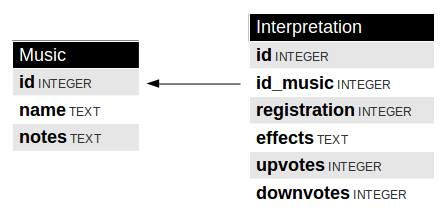
\includegraphics[width=\textwidth]{images/tree.jpg}
\caption{Árvore da base de dados, com as tabelas da música (\emph{musics}) e interpretação (\emph{interpretation}).}
\label{tree}
\end{figure}

Dentro do ficheiro que cria a base de dados, há uma condição que verifica se se encontra criada a base de dados, ou então se é o próprio programa que a cria, através do ficheiro \emph{create.txt}.

\vspace{5mm}
\begin{lstlisting}
if not os.path.isfile('songs.db'):
	
	if not os.path.isfile('create.txt'):
		print 'We need a database to run the program. We don\'t have one, so we need a "create.txt" file to create the library. Copy a valid "create.txt" file to this folder and reopen the program.'
		exit(1)
		
	db = sql.connect('songs.db')
	
	createDBfile = open('create.txt', 'r')
	
	for line in createDBfile:
		db.execute(line)	
	
	db.commit()
	createDBfile.close()
	db.close()
\end{lstlisting}
\vspace{5mm}

Dentro do próprio programa, existe uma série de funções que permite efectuar operações na base de dados.

\vspace{5mm}
\begin{lstlisting}
def is_mobile(request):
    ismobile = False

    if request.headers.has_key('User-Agent'):
        user_agent = request.headers['User-Agent']

        # Test common mobile values.
        patterns = "(xoom|up.browser|up.link|mmp|symbian|smartphone|phone|tablet|midp|wap|windows ce|pda|mobile|mini|palm|netfront|nokia)"

        patt_compiled = re.compile(patterns, re.IGNORECASE)
        match = patt_compiled.search(user_agent)

        if match:
           ismobile = True

    return ismobile
\end{lstlisting}
\vspace{5mm}

Esta função, permite que a base de dados ao comunicar com o servidor, permite saber se o dispositivo onde vai ser executado a aplicação é um dispositivo móvel ou um computador, sendo depois mostrado ao utilizador a interface correspondente.  

\vspace{5mm}
\begin{lstlisting}
def create_song(name, notes):
	command = 'INSERT INTO musics(name, notes) VALUES("' + name + '", "' + notes + '")'
	db.execute(command)
	db.commit()
\end{lstlisting}
\vspace{5mm}

A função acima descrita permite criar uma nova música na tabela das músicas, sendo que a cada nova música adicionada irá haver uma \textbf{id} que lhes é atribuida, facilitando desta forma identificar a música mais facilmete caso seja necessário fazer alterações. Para criar uma nova interpretação seguem-se os mesmos padrões do exemplo anterior.

Tal como é possível adicionar novas músicas, também se pode visualizar o conteúdo de uma tabela, neste caso, o conteúdo da \textbf{interpretations}, através do exemplo seguinte:

\vspace{5mm}
\begin{lstlisting}
def get_all_notes():
	command = 'SELECT * FROM musics'
	result = db.execute(command)
	rows = result.fetchall()
	d = []
	for row in rows:
		name = {"id":row[0],"name":row[1],"notes":row[2]}
		d.append(name)

	return d
\end{lstlisting}
\vspace{5mm}

Para ser possível actualizar o número de votos, neste caso positivos, sendo o mesmo método aplicado no número de gostos negativos, recorreu-se ao seguinte código. Esta função vai mostrar os votos positivos de uma determinada interpretação, sendo o valor guardado numa variável onde será incrementado em mais uma unidade. Após isso executa-se um novo comando e actualiza-se o número de gostos positivos para o novo valor.  

\vspace{5mm}
\begin{lstlisting}
def add_upvotes(ID):
	command = 'SELECT upvotes FROM interpretations WHERE id = ' + str(ID)
	result = db.execute(command)
	result = result.fetchone()
	result = result[0] + 1
	command = 'UPDATE interpretations SET upvotes = "' + str(result) + '" WHERE id = ' + str(ID)
	db.execute(command)
	db.commit()

\end{lstlisting}
\vspace{5mm}


\vspace{5mm}
\begin{lstlisting}

def last_id_interpretations():
	try:
		result = db.execute("SELECT id FROM interpretations")
		rows = result.fetchall()
		x = []
		for row in rows:
			x.append(row[0])

		return x[len(x)-1]+1
	except IndexError, e:
		return 1

\end{lstlisting}

Como se pode verificar pelo código acima descrito, esta função vai tentar apanhar uma exceção, quando mostra todas as \textbf{id's} da tabela interpretações, guardando-as numa lista, verificando se a sequência está dentro do intervalo, e caso não esteja, a exceção é gerada. 
